\documentclass{beamer}

\usepackage[T2A]{fontenc}
\usepackage[utf8]{inputenc}
\usepackage[english,russian]{babel}
\input{settings.tex}


\title{Коническое программирование}
\subtitle{\mycoursetitle, лекция 7}
\author{Сергей Савин}
\centering
\date{\mydate}



\begin{document}
\maketitle


%\begin{frame}{Content}
%
%\begin{itemize}
%\item  Quadratically constrained quadratic programming (QCQP)
%\item  Second-order cone programming
%\item  Friction cone as an SOCP
%\end{itemize}
%
%\end{frame}
\begin{frame}{QCQP}
	
	{\huge Квадратично ограниченное квадратичное программирование}
	
\end{frame}



\begin{frame}{Квадратично ограниченное квадратичное программирование}
	\begin{flushleft}
		
		Общий вид выпуклой задачи квадратично ограниченного квадратичного программирования (QCQP) приведён ниже:
		
		%
		\begin{equation}
			\begin{aligned}
				& \underset{\mathbf{x}}{\text{minimize}}
				& & \mathbf{x}^\top \mathbf{P}_0 \mathbf{x} + \mathbf{q}_0^\top\mathbf{x}, \\
				& \text{subject to:}
				& & \begin{cases}
					\mathbf{x}^\top \mathbf{P}_i \mathbf{x} + \mathbf{q}_i^\top\mathbf{x} + r_i \leq 0, \\
					\mathbf{F}\mathbf{x} = \mathbf{g}.
				\end{cases}
			\end{aligned}
		\end{equation}
		
		где $\mathbf{P}_i$ положительно определены.
		
	\end{flushleft}
\end{frame}



\begin{frame}{QCQP - Область определения}
	\begin{flushleft}
		
		Область определения выпуклой QCQP без ограничений-равенств и без вырожденных неравенств представляет собой пересечение эллипсов:
		
		\begin{figure} [h!]
			\begin{center}
				\input{fig_1.tex}
			\end{center} 
		\end{figure}
		
	\end{flushleft}
\end{frame}



\begin{frame}{От QCQP к QP и LP}
	\begin{flushleft}
		
		Положим $\mathbf{P}_i = \mathbf{0}$ — и получим QP.
		%
		\begin{equation}
			\begin{aligned}
				& \underset{\mathbf{x}}{\text{minimize}}
				& & \mathbf{x}^\top \mathbf{P}_0 \mathbf{x} + \mathbf{q}_0^\top\mathbf{x}, \\
				& \text{subject to:}
				& & \begin{cases}
					\begin{bmatrix} 
						\mathbf{q}_1^\top \\ ... \\ \mathbf{q}_n^\top
					\end{bmatrix} 
					\mathbf{x} \leq
					\begin{bmatrix} 
						-r_1 \\ ... \\ -r_n
					\end{bmatrix} \\
					\mathbf{F}\mathbf{x} = \mathbf{g}.
				\end{cases}
			\end{aligned}
		\end{equation}
		
		Положим $\mathbf{P}_0 = \mathbf{0}$ — и получим LP.
		
	\end{flushleft}
\end{frame}


\begin{frame}{SOCP}
	
	{\huge Коническое программирование второго порядка}
	
\end{frame}




\begin{frame}{2-норма, 1}
	\begin{flushleft}
		
		Рассмотрим 2-норму как функцию $f(\bo{x}): \ \R^n \rightarrow \R$:
		
		\begin{align}
			f(\bo{x}) = || \bo{x} ||_2
			\\
			f(\bo{x}) = \sqrt{ \sum_{i=1}^n x_i^2 }
		\end{align}
		
	\end{flushleft}
\end{frame}


\begin{frame}{2-норма, 2}
	\begin{flushleft}
		
		Мы можем описать 2-норму как поверхность в пространстве $\mathcal S \subset \R^{n+1}$:
		
		\begin{align}
			\mathcal S = \{  (J, \bo{x}): \ J = || \bo{x} ||_2 \}
		\end{align}		
		
		\begin{figure}
			\centering
			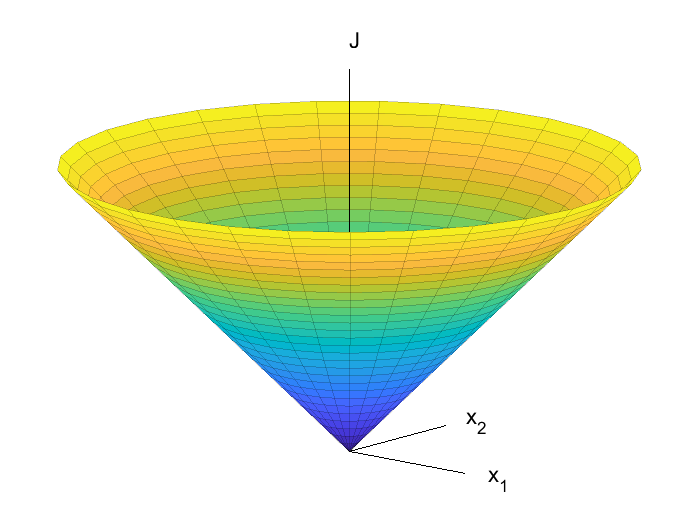
\includegraphics[width=0.7\linewidth]{norm}
			%			\caption{}
			\label{fig:norm}
		\end{figure}
		
	\end{flushleft}
\end{frame}



\begin{frame}{Конус}
	\begin{flushleft}
		
		Форма поверхности $\mathcal S = \{  (J, \bo{x}): \ J = || \bo{x} ||_2 \}$ является границей \emph{конуса}. Наблюдаем следующие свойства конуса:
		
		\begin{itemize}
			\item Конус имеет вершину (остриё).
			
			\item Конус замкнут относительно положительного масштабирования: если $( \bo{x}, \| \bo{x}\| )$ принадлежит конусу, то $( \alpha \bo{x}, \|  \alpha\bo{x}\| )$ также принадлежит этому конусу.
			
			\item Поперечные сечения, перпендикулярные оси, являются сферами.
		\end{itemize}
		
		
	\end{flushleft}
\end{frame}





\begin{frame}{Конус второго порядка, 1}
	\begin{flushleft}
		
		Ограничение конуса второго порядка имеет следующий вид:
		
		\begin{equation}
			||\bo{z}|| \leq t
		\end{equation}
		%
		где $\bo{z}$ и $t$ — переменные. С помощью аффинных преобразований (аффинной замены переменных) мы можем переписать его в более общем виде:
		
		\begin{equation}
			||\bo{A}\bo{x}+\bo{b}|| \leq \bo{c}\T \bo{x} + d
		\end{equation}
		%
		где $\bo{A} \in \R^{m, n}$, $\bo{b}\in \R^{m}$, $\bo{c} \in \R^{n}$ и $d \in \R$.
		
		\bigskip
		
		Для допустимости правая часть должна быть неотрицательной: $\bo{c}\T \bo{x} + d \geq 0$.
		
	\end{flushleft}
\end{frame}


\begin{frame}{Конус второго порядка, 2}
	\begin{flushleft}
		
		Ограничение $||\bo{A}\bo{x}+\bo{b}|| \leq \bo{c}\T \bo{x} + d$ описывает аффинное преобразование конуса. Его поверхность является пересечением двух поверхностей в $\R^{n+1}$: 
		
		\begin{align}
			y = ||\bo{A}\bo{x}+\bo{b}|| \\
			y = \bo{c}\T \bo{x} + d
		\end{align}
		
		Первая — это конус, а вторая — плоскость. 
		
		
	\end{flushleft}
\end{frame}






\begin{frame}{Роль свободной константы, 1}
	\begin{flushleft}
		
		Коническое сечение — это пересечение плоскости и двойного конуса. Типичные конические сечения показаны ниже:
		
		\begin{figure}
			\centering
			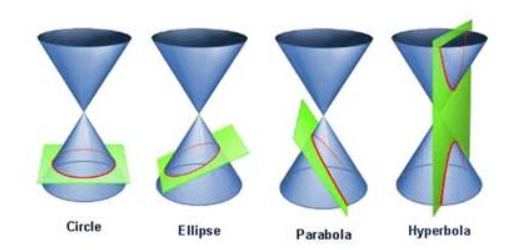
\includegraphics[width=0.7\linewidth]{cones}
			\label{fig:cones}
		\end{figure}
		
		Как мы видим, они представляют собой эллипсоид и параболу. Чтобы они представляли конус, плоскость $S$ должна проходить через вершину конуса $J$. Это можно достичь соответствующим выбором константы $d$, которая сдвигает $S$ вверх или вниз.
		
	\end{flushleft}
\end{frame}



\begin{frame}{Роль свободной константы, 2}
	\begin{flushleft}
		
		Поверхность аффинного конуса имеет вид:
		%
		\begin{equation}
			||\bo{A}\bo{x}+\bo{b}|| = \bo{c}\T \bo{x} + d
		\end{equation}
		
		мы можем найти точку вершины; она соответствует обращению в ноль как правой, так и левой части:
		
		\begin{equation}
			\begin{cases}
				\bo{A}\bo{x}+\bo{b} = 0 \\
				\bo{c}\T \bo{x} + d = 0
			\end{cases}
		\end{equation}
		
		При матрице $\bo{A}$ полного ранга решение имеет вид $\bo{x} = -\bo{A}^{-1}\bo{b}$. Система будет выполнена, если:
		
		\begin{equation}
			-\bo{c}\T \bo{A}^{-1}\bo{b} + d = 0
		\end{equation}
		
		
	\end{flushleft}
\end{frame}







\begin{frame}{Коническое программирование второго порядка (SOCP)}
	\framesubtitle{Общий вид}
	\begin{flushleft}
		
		
		Общий вид задачи конического программирования второго порядка (SOCP):
		
		%
		\begin{equation}
			\begin{aligned}
				& \underset{\mathbf{x}}{\text{minimize}}
				& & \mathbf{f}^\top\mathbf{x}, \\
				& \text{subject to}
				& & \begin{cases}
					||\mathbf{A}_i\mathbf{x} + \mathbf{b}_i||_2 \leq 
					\mathbf{c}_i^\top \mathbf{x} + d_i, \\
					\mathbf{F}\mathbf{x} = \bo{g}.
				\end{cases}
			\end{aligned}
		\end{equation}
		
		LP, QP и выпуклые QCQP являются подмножествами SOCP.
		
	\end{flushleft}
\end{frame}








\begin{frame}{Коническое программирование второго порядка}
	\framesubtitle{Частные случаи}
	\begin{flushleft}
		
		Мы можем записать задачу, где область определения — шар, как SOCP:
		%
		\begin{equation}
			\begin{aligned}
				& \underset{\mathbf{x}}{\text{minimize}}
				& & \mathbf{f}^\top\mathbf{x}, \\
				& \text{subject to}
				& & ||\mathbf{x}||_2 \leq d
			\end{aligned}
		\end{equation}
		
		\bigskip
		
		То же самое для эллипсоидальных ограничений:
		%
		\begin{equation}
			\begin{aligned}
				& \underset{\mathbf{x}}{\text{minimize}}
				& & \mathbf{f}^\top\mathbf{x}, \\
				& \text{subject to}
				& & ||\mathbf{A}_i\mathbf{x}||_2 \leq d_i
			\end{aligned}
		\end{equation}
		
	\end{flushleft}
\end{frame}




\begin{frame}{Пример — планирование пути}
	\begin{flushleft}
		
		Рассмотрим задачу планирования пути: найти последовательность точек $\bo{x}_i$, начинающуюся в $\bo{x}_0$, строящую кратчайший путь до целевой точки $\bo{x}_g$, такую, что соседние точки находятся не дальше $h$ друг от друга.
		
		\bigskip
		
		\textbf{Решение}. 
		Задача принимает вид:
		
		
		%
		\begin{equation}
			\begin{aligned}
				& \underset{\bo{x}_1, ..., \bo{x}_n}{\text{minimize}}
				& & \sum_{i = 1}^{n} (\bo{x}_i - \bo{x}_{i+1})\T (\bo{x}_i - \bo{x}_{i+1}), \\
				& \text{subject to}
				& &
				\begin{cases}
					||\bo{x}_i - \bo{x}_{i+1} || \leq h, \ \ i \in {0, 1, 2, ...., n} \\
					\bo{x}_n = \bo{x}_g
				\end{cases}
			\end{aligned}
		\end{equation}
		
	\end{flushleft}
\end{frame}




\begin{frame}{От SOCP к QCQP, 1}
	\begin{flushleft}
		
		Положим $\mathbf{c}_i = 0$ и заметим, что $||\mathbf{A}_i\mathbf{x} + \mathbf{b}_i||_2 \leq d_i$ эквивалентно $(\mathbf{A}_i\mathbf{x} + \mathbf{b}_i)^\top (\mathbf{A}_i\mathbf{x} + \mathbf{b}_i) \leq d_i^2$ (поскольку из первого неравенства следует неотрицательность $d_i$).
		
		\bigskip
		%
		\begin{equation}
			\begin{aligned}
				& \underset{\bo{x}}{\text{minimize}}
				& & \bo{f}^\top\bo{x}, \\
				& \text{subject to}
				& & \begin{cases}
					\bo{x}^\top \bo{A}_i^\top \bo{A}_i \bo{x} + 
					2 \bo{b}_i^\top \bo{A}_i\bo{x} + 
					\bo{b}_i^\top \bo{b}_i  \leq d_i^2\\
					\bo{F}\bo{x} = \bo{g}.
				\end{cases}
			\end{aligned}
		\end{equation}
		
	\end{flushleft}
\end{frame}




\begin{frame}{От SOCP к QCQP, 2}
	\begin{flushleft}
		
		
		Теперь сделаем целевой функционал квадратичным:
		%
		\begin{equation}
			\begin{aligned}
				& \underset{\bo{x}, t}{\text{minimize}}
				& & t, \\
				& \text{subject to}
				& & \begin{cases}
					\bo{x}^\top \bo{A}_0^\top \bo{A}_0 \bo{x} + 
					2 \bo{b}_0^\top \bo{A}_0\bo{x} + 
					\bo{b}_0^\top \bo{b}_0  \leq t\\
					\bo{x}^\top \bo{A}_i^\top \bo{A}_i \bo{x} + 
					2 \bo{b}_i^\top \bo{A}_i\bo{x} + 
					\bo{b}_i^\top \bo{b}_i  \leq d_i^2\\
					\bo{F}\bo{x} = \bo{g}.
				\end{cases}
			\end{aligned}
		\end{equation}
		
		Что эквивалентно:
		%
		\begin{equation}
			\begin{aligned}
				& \underset{\bo{x}}{\text{minimize}}
				& & \mathbf{x}^\top \mathbf{H} \mathbf{x} + \mathbf{f}^\top\mathbf{x}, \\
				& \text{subject to}
				& & \begin{cases}
					\bo{x}^\top \bo{A}_i^\top \bo{A}_i \bo{x} + 
					2 \bo{b}_i^\top \bo{A}_i\bo{x} + 
					\bo{b}_i^\top \bo{b}_i  \leq d_i^2\\
					\bo{F}\bo{x} = \bo{g}.
				\end{cases}
			\end{aligned}
		\end{equation}
		
		При условии, что $\bo{A}_0 = \sqrt{\bo{H}}$, и $\bo{b}_0 = 0.5 \bo{A}_0^{-1} \mathbf{f}$.
		
	\end{flushleft}
\end{frame}

\begin{frame}
	\centerline{\huge Конус трения как SOC}
\end{frame}


\begin{frame}{Трение в 3D, 1}
	\begin{flushleft}
		
		Сила трения $\bo{f}_\tau$ вместе с нормальной реакцией $\bo{f}_n$ образуют контактную силу реакции $\bo{f}_R$:
		
		\begin{align}
			\bo{f}_R = \bo{f}_n + \bo{f}_\tau
		\end{align}
		
		Мы можем представить силу реакции в базисе $\bo{B}$, образованном объединением нормального направления $\bo{n}$ и двух касательных направлений $\bo{t}_1$, $\bo{t}_2$.
		
		\begin{align}
			\bo{f}_R
			=
			\bo{B}
			\begin{bmatrix}
				f_n \\ f_{\tau, 1} \\ f_{\tau, 2}
			\end{bmatrix}
			=
			\begin{bmatrix}
				\bo{n} & \bo{t}_1 & \bo{t}_2
			\end{bmatrix}
			\begin{bmatrix}
				f_n \\ f_{\tau, 1} \\ f_{\tau, 2}
			\end{bmatrix}
		\end{align}
		
		
		
	\end{flushleft}
\end{frame}



\begin{frame}{Трение в 3D, 2}
	\begin{flushleft}
		
		Мы можем доказать, что $f_n = \bo{n}\T \bo{f}_R$:
		
		\begin{align}
			\bo{n}\T \bo{f}_R = 
			\bo{n}\T
			\begin{bmatrix}
				\bo{n} & \bo{t}_1 & \bo{t}_2
			\end{bmatrix}
			\begin{bmatrix}
				f_n \\ f_{\tau, 1} \\ f_{\tau, 2}
			\end{bmatrix}
			=
			\begin{bmatrix}
				1 & 0 & 0
			\end{bmatrix}
			\begin{bmatrix}
				f_n \\ f_{\tau, 1} \\ f_{\tau, 2}
			\end{bmatrix}
			=
			f_n 
		\end{align}
		
		
		Мы можем доказать, что $\begin{bmatrix}
			f_{\tau, 1} \\ f_{\tau, 2}
		\end{bmatrix} = 
		\begin{bmatrix}
			\bo{t}_1 & \bo{t}_2
		\end{bmatrix}\T \bo{f}_R$:
		
		\begin{align}
			\begin{bmatrix}
				\bo{t}_1 & \bo{t}_2
			\end{bmatrix}\T \bo{f}_R = 
			\begin{bmatrix}
				\bo{t}_1 & \bo{t}_2
			\end{bmatrix}\T
			\begin{bmatrix}
				\bo{n} & \bo{t}_1 & \bo{t}_2
			\end{bmatrix}
			\begin{bmatrix}
				f_n \\ f_{\tau, 1} \\ f_{\tau, 2}
			\end{bmatrix}
			= \\
			=
			\begin{bmatrix}
				0 & 1 & 0 \\
				0 & 0 & 1
			\end{bmatrix}
			\begin{bmatrix}
				f_n \\ f_{\tau, 1} \\ f_{\tau, 2}
			\end{bmatrix}
			=
			\begin{bmatrix}
				f_{\tau, 1} \\ f_{\tau, 2}
			\end{bmatrix}
		\end{align}
		
		
	\end{flushleft}
\end{frame}




\begin{frame}{Представления конуса трения, 1}
	\begin{flushleft}
		
		Мы можем записать ограничение конуса трения следующим образом:
		
		\begin{equation}
			\sqrt{f_{\tau, 1}^2 + f_{\tau, 2}^2} \leq \mu f_n
		\end{equation}
		
		где $\mu$ — коэффициент трения, $f_\tau$ — величина силы трения, а $f_n$ — величина нормальной силы реакции.
		
		\bigskip
		
		Мы можем описать это как \emph{покомпонентное описание}. Простота этого описания делает его довольно привлекательным.
		
		
	\end{flushleft}
\end{frame}


\begin{frame}{Представления конуса трения, 2}
	\begin{flushleft}
		
		Можно переписать то же самое ограничение в виде:
		
		\begin{equation}
			\left|\left| \begin{bmatrix}
				\bo{t}_1 & \bo{t}_2
			\end{bmatrix}\T
			\bo{f}_R \right|\right| 
			\leq \mu \bo{n}\T \bo{f}_R
		\end{equation}
		
		Назовём это \emph{векторным описанием}. Преимущество этого описания — использование одной векторной переменной $\bo{f}_R$. Оно принимает форму ограничения конуса второго порядка (SOC).
		
		\bigskip
		
		Обратите внимание, что $\bo{t}_1$ и $\bo{t}_2$ обычно не заданы и могут быть выбраны произвольно, с точностью до поворота. Мы можем найти их как левое нуль-пространство нормального вектора: $\bo{T} = \begin{bmatrix}
			\bo{t}_1 & \bo{t}_2
		\end{bmatrix} = \text{null}(\bo{n}\T)$: 
		
		\begin{equation}
			|| \bo{T}\T\bo{f}_R ||
			\leq \mu \bo{n}\T \bo{f}_R
		\end{equation}
		
	\end{flushleft}
\end{frame}



\begin{frame}{Представления конуса трения, 3}
	\begin{flushleft}
		
		То же самое можно сделать с помощью проекторов:
		
		
		\begin{equation}
			|| (\bo{I} - \bo{n}\bo{n}\T) \bo{f}_R ||
			\leq \mu \bo{n}\T \bo{f}_R
		\end{equation}
		
		
		
	\end{flushleft}
\end{frame}




\begin{frame}{Домашнее задание}
	\begin{flushleft}
		
		\begin{itemize}
			\item Реализуйте программу, которая находит крайнюю правую точку пересечения двух эллипсоидов; визуализируйте задачу и решение.
			
			\item Постройте конус по заданному направлению и заданному углу при вершине.
		\end{itemize}
		
		
		
		
	\end{flushleft}
\end{frame}




\myqrframe



\begin{frame}
	\centerline{\huge Appendix A - canonical form}
\end{frame}


\begin{frame}{Canonical form, degenerate cone marix, 1}
	\begin{flushleft}
		
		Consider the following SOC constraint:
		
		\begin{equation}
			\label{eq:SOC}
			||\mathbf{A}\mathbf{x} + \mathbf{b}||_2 \leq 
			\mathbf{c}^\top \mathbf{x} + d
		\end{equation}
		
		Let us consider a special case when $\mathbf{x} \in \R^n$, $\mathbf{A} \in \R^{(n-1) \times n}$ and $\text{rank}\left(\begin{bmatrix}
			\mathbf{A} \\ \mathbf{c}^\top
		\end{bmatrix}\right) = n$. Then we can introduce the following substitution:
		
		\begin{equation}
			\xi = \begin{bmatrix}
				\mathbf{A} \\ \mathbf{c}^\top
			\end{bmatrix}
			\mathbf{x} + 
			\begin{bmatrix}
				\mathbf{b} \\ d
			\end{bmatrix}, 
			\ \ \ 
			\mathbf{I} = 
			\begin{bmatrix}
				\mathbf{E} \\ \mathbf{e}^\top
			\end{bmatrix}
		\end{equation}
		%
		where $\mathbf{I} \in\R^{n, n}$ is an identity matrix. Then constraint \eqref{eq:SOC} becomes:
		
		\begin{equation}
			||\mathbf{E}\xi||_2 \leq 
			\mathbf{e}^\top \xi
		\end{equation}
		
	\end{flushleft}
\end{frame}


\begin{frame}{Canonical form, degenerate cone marix, 2}
	\begin{flushleft}
		
		Notice that $||\mathbf{E}\xi||_2 \leq 
		\mathbf{e}^\top \xi$ is equivalent to:
		
		\begin{equation}
			\sum\limits_{i=1}^{n-1}\xi_i^2 \leq \xi_n^2 
		\end{equation}
		%	
		which is a standard form of a cone. A map back from $\xi$ to $\mathbf{x}$ is given as:
		
		\begin{equation}
			\mathbf{x} = \begin{bmatrix}
				\mathbf{A} \\ \mathbf{c}^\top
			\end{bmatrix}^{-1}
			\left(
			\xi - 
			\begin{bmatrix}
				\mathbf{b} \\ d
			\end{bmatrix}
			\right)
		\end{equation}
		
	\end{flushleft}
\end{frame}



\begin{frame}
	\centerline{\huge Appendix B - plotting cones}
\end{frame}


\begin{frame}{Plotting level sets, 1}
	\begin{flushleft}
		
		To plot a cone it is convenient to first use change of coordinates $\bo{y} = \bo{A}\bo{x}+\bo{b}$, meaning $\bo{x} =\bo{A}^{-1} (\bo{y} - \bo{b})$, giving us SOC:
		%
		\begin{equation}
			||\bo{y}|| = \bo{c}\T \bo{A}^{-1} (\bo{y} - \bo{b}) + d
		\end{equation}
		
		Note that $d - \bo{c}\T \bo{A}^{-1}\bo{b} = 0$ for a cone with a tip; so SOC becomes:
		%
		\begin{equation}
			||\bo{y}|| = \bo{c}\T \bo{A}^{-1} \bo{y}
		\end{equation}
		
		To plot level sets of this cone we choose height of the level set $h$ and pick point $\bo{y}_h = h \frac{\bo{A}^{-T} \bo{c}}{\bo{c}\T \bo{A}^{-1}\bo{A}^{-T} \bo{c}}$; we note that $\bo{c}\T \bo{A}^{-1} \bo{y}_h = h$. Then we consider points on the plane $\mathcal P$ orthogonal to $\bo{c}\T \bo{A}^{-1}$ and passing through $\bo{y}_h$:
		
		\begin{equation}
			\mathcal P = {\bo{y}_h + \bo{T}\bo{z}: \  \forall \bo{z}}
		\end{equation}
		%
		where $\bo{T} = \text{null}(\bo{c}\T \bo{A}^{-1})$, so $\bo{c}\T \bo{A}^{-1} \bo{T} = 0$.
		
	\end{flushleft}
\end{frame}


\begin{frame}{Plotting level sets, 2}
	\begin{flushleft}
		
		Since  SOC becomes:
		%
		\begin{equation}
			||\bo{y}_h + \bo{T}\bo{z}|| = h
		\end{equation}
		
		Since $\bo{y}_h$ and $\bo{T}\bo{z}$ are orthogonal, it is equivalent to:
		%
		\begin{equation}
			||\bo{T}\bo{z}|| = g
		\end{equation}
		%
		where $g = \sqrt{ h^2 - \bo{y}_h\T\bo{y}_h }$. In the 3D case, this is a circle with radius $g$. We can find $N$ consecutive evenly spaced points of this circle, resulting in the next sequence of $\bo{y}_l$:
		
		\begin{align}
			\bo{y}_l &= \bo{y}_h + \bo{T}
			\begin{bmatrix}
				g\cos(\varphi) \\ -g\sin(\varphi)
			\end{bmatrix}, \ \ \ \varphi = 0, \ \frac{2\pi}{N},\ 2\frac{2\pi}{N}, \ ..., \ 2\pi 
			\\
			\bo{x}_l  &=\bo{A}^{-1} (\bo{y}_l - \bo{b})
		\end{align}
		
		The center of the ellipsoid representing this level set lies at the point $\bo{x} =\bo{A}^{-1} (\bo{y}_h - \bo{b})$.
		
	\end{flushleft}
\end{frame}



\begin{frame}{Plotting level sets, 3}
	\begin{flushleft}
		
		
		\begin{figure}
			\centering
			\begin{subfigure}[b]{0.45\textwidth}
				\centering
				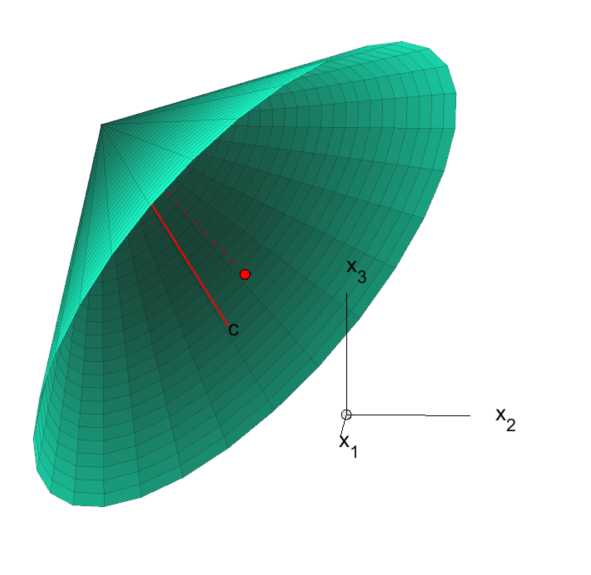
\includegraphics[width=\textwidth]{plotted1}
			\end{subfigure}
			\hfill
			\begin{subfigure}[b]{0.45\textwidth}
				\centering
				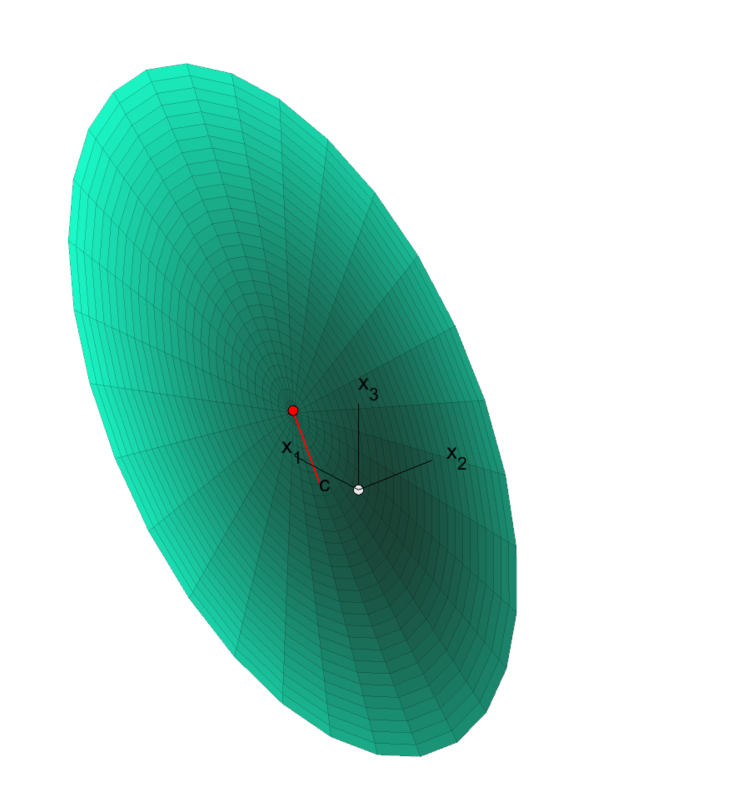
\includegraphics[width=\textwidth]{plotted2}
			\end{subfigure}
			\caption{Cone. Dashed line - centers of level-sets.}
		\end{figure}
		
	\end{flushleft}
\end{frame}



\begin{frame}
	\centerline{\huge Appendix C -}
	
	\bigskip
	
	\centerline{\huge Transforming ellipsoid}
	\centerline{\huge to the canonical form}
\end{frame}




\begin{frame}{Turning ellipsoid to the canonical form (1)}
	\begin{flushleft}
		
		Can we re-write the expression $\mathbf{x}^\top \mathbf{P} \mathbf{x} + \mathbf{q}^\top\mathbf{x} + r \leq 0$ as a canonical form ellipsoid:
		
		\begin{equation}
			\frac{z_1^2}{m_1^2} + \frac{z_2^2}{m_2^2} + ... + 
			\frac{z_n^2}{m_n^2} \leq 1
		\end{equation}
		
		We start by proposing a substitution $\bo{x}_0 = - \frac{1}{2}\bo{P}^{-1}\bo{q}$ and $-d = r - \bo{x}_0\T \bo{P} \bo{x}_0$. We can prove that: $(\bo{x} - \bo{x}_0)\T \bo{P}(\bo{x} - \bo{x}_0) - d =
		\mathbf{x}^\top \mathbf{P} \mathbf{x} + \mathbf{q}^\top\mathbf{x} + r$
		
		\begin{align}
			(\bo{x} - \bo{x}_0)\T \bo{P}(\bo{x} - \bo{x}_0) - d =
			\\
			= \bo{x}\T\bo{P}\bo{x} - 2\bo{x}_0\T\bo{P}\bo{x} + \bo{x}_0\T\bo{P}\bo{x}_0 - d &=
			\\
			= \bo{x}\T\bo{P}\bo{x} + 2\left(\textcolor{mydarkblue}{\frac{1}{2}\bo{P}^{-1}\bo{q}}\right)\T\bo{P}\bo{x} + \bo{x}_0\T\bo{P}\bo{x}_0 + \textcolor{mydarkblue}{r - \bo{x}_0\T \bo{P} \bo{x}_0} &=
			\\
			= \bo{x}\T\bo{P}\bo{x} + \bo{q}\T \bo{x} + r.
		\end{align}
		
	\end{flushleft}
\end{frame}



\begin{frame}{Turning ellipsoid to the canonical form (2)}
	\begin{flushleft}
		
		Thus our original expression became:
		%
		\begin{align}
			(\bo{x} - \bo{x}_0)\T \bo{P}(\bo{x} - \bo{x}_0) - d \leq 0
		\end{align}
		%
		We define $\bo{A} = \sqrt{\bo{P}}$ with SVD decomposition $\bo{A} = \bo{U} \Sigma \bo{V}\T$. Defining $\bo{z} = \bo{V}\T (\bo{x} - \bo{x}_0)$ we get:
		%
		\begin{align}
			(\bo{x} - \bo{x}_0)\T \bo{A}\T\bo{A}(\bo{x} - \bo{x}_0) - d \leq 0 
			\\
			(\bo{x} - \bo{x}_0)\T  \bo{V} \Sigma \bo{U}\T  \bo{U} \Sigma \bo{V}\T(\bo{x} - \bo{x}_0) - d \leq 0 
			\\
			(\bo{x} - \bo{x}_0)\T  \bo{V} \Sigma^2 \bo{V}\T(\bo{x} - \bo{x}_0) - d \leq 0
			\\
			\bo{z}\T   \Sigma^2 \bo{z} - d \leq 0
			\\
			\sum z_i^2 \sigma_i^2  \leq d
		\end{align}
		%
		Defining $1/m_i^2 = \sigma_i^2 / d$ we get:
		%
		\begin{equation}
			\frac{z_1^2}{m_1^2} + \frac{z_2^2}{m_2^2} + ... + 
			\frac{z_n^2}{m_n^2} \leq 1
		\end{equation}
		
		
	\end{flushleft}
\end{frame}


\end{document}
